\documentclass{standalone}
\usepackage{tikz}
\usetikzlibrary{patterns, positioning}
\usepackage[sfdefault]{ClearSans} %% option 'sfdefault' activates Clear Sans as the default text font
\usepackage[T1]{fontenc}

\begin{document}
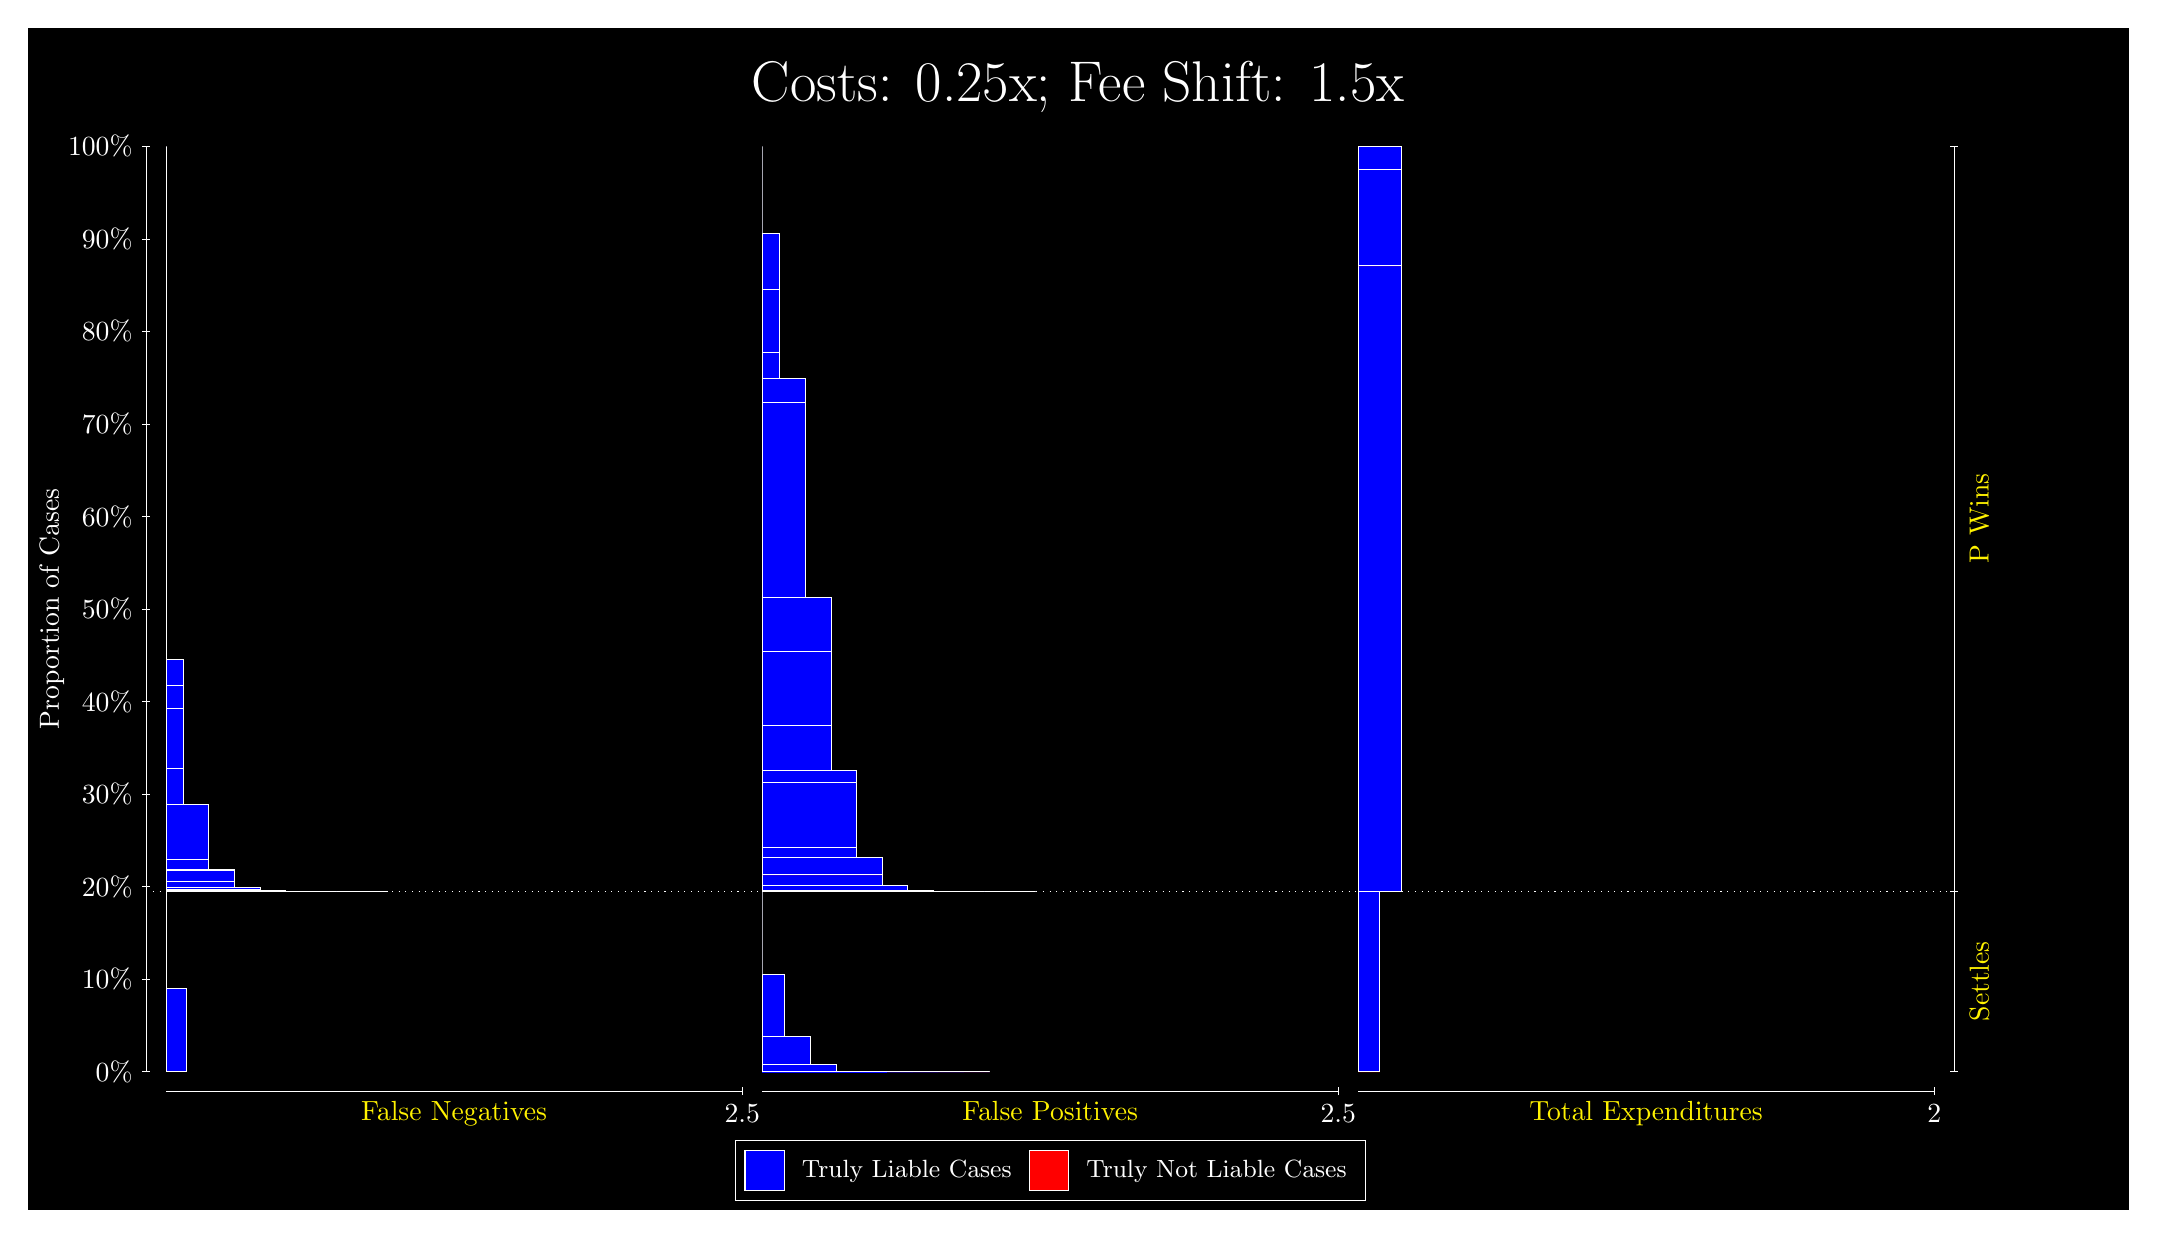
\begin{tikzpicture}
\draw[fill=black] (0,0) rectangle (26.667,15);
\draw[text=white] (0,13.5) rectangle (26.667,15) node[midway] {\huge Costs: 0.25x; Fee Shift: 1.5x};
\draw[white, very thin] (1.5,1.75) -- (1.5,13.5);
\node[rotate=90, text=white, anchor=center] at (0.3, 7.625) {Proportion of Cases};
\draw[white, very thin] (1.45,1.75) -- (1.55,1.75);
\node[text=white, anchor=east] at (1.45, 1.75) {0\%};
\draw[white, very thin] (1.45,2.925) -- (1.55,2.925);
\node[text=white, anchor=east] at (1.45, 2.925) {10\%};
\draw[white, very thin] (1.45,4.1) -- (1.55,4.1);
\node[text=white, anchor=east] at (1.45, 4.1) {20\%};
\draw[white, very thin] (1.45,5.275) -- (1.55,5.275);
\node[text=white, anchor=east] at (1.45, 5.275) {30\%};
\draw[white, very thin] (1.45,6.45) -- (1.55,6.45);
\node[text=white, anchor=east] at (1.45, 6.45) {40\%};
\draw[white, very thin] (1.45,7.625) -- (1.55,7.625);
\node[text=white, anchor=east] at (1.45, 7.625) {50\%};
\draw[white, very thin] (1.45,8.8) -- (1.55,8.8);
\node[text=white, anchor=east] at (1.45, 8.8) {60\%};
\draw[white, very thin] (1.45,9.975) -- (1.55,9.975);
\node[text=white, anchor=east] at (1.45, 9.975) {70\%};
\draw[white, very thin] (1.45,11.15) -- (1.55,11.15);
\node[text=white, anchor=east] at (1.45, 11.15) {80\%};
\draw[white, very thin] (1.45,12.325) -- (1.55,12.325);
\node[text=white, anchor=east] at (1.45, 12.325) {90\%};
\draw[white, very thin] (1.45,13.5) -- (1.55,13.5);
\node[text=white, anchor=east] at (1.45, 13.5) {100\%};

\draw[white, very thin] (24.457,1.75) -- (24.457,13.5);
\draw[white, very thin] (24.407,1.75) -- (24.507,1.75);
\node[anchor=west] at (24.407, 1.75) {};
\draw[white, very thin] (24.407,4.0413) -- (24.507,4.0413);
\node[anchor=west] at (24.407, 4.0413) {};
\draw[white, very thin] (24.407,13.5) -- (24.507,13.5);
\node[anchor=west] at (24.407, 13.5) {};

\draw[white, very thin, fill=blue] (1.75,1.75) rectangle (2.0062,2.8115);
\draw[white, very thin, fill=red] (1.75,2.8115) rectangle (1.75,2.8115);
\draw[white, very thin, fill=blue] (1.75,2.8115) rectangle (1.75,4.0413);
\draw[white, very thin, fill=blue] (1.75,4.0413) rectangle (4.5678,4.0413);
\draw[white, very thin, fill=blue] (1.75,4.0413) rectangle (4.2425,4.0413);
\draw[white, very thin, fill=blue] (1.75,4.0413) rectangle (4.2425,4.0413);
\draw[white, very thin, fill=blue] (1.75,4.0413) rectangle (3.9172,4.0413);
\draw[white, very thin, fill=blue] (1.75,4.0413) rectangle (3.5919,4.0416);
\draw[white, very thin, fill=blue] (1.75,4.0416) rectangle (3.2666,4.0443);
\draw[white, very thin, fill=blue] (1.75,4.0443) rectangle (3.2666,4.0463);
\draw[white, very thin, fill=blue] (1.75,4.0463) rectangle (2.9413,4.0634);
\draw[white, very thin, fill=blue] (1.75,4.0634) rectangle (2.9413,4.0882);
\draw[white, very thin, fill=blue] (1.75,4.0882) rectangle (2.6161,4.172);
\draw[white, very thin, fill=blue] (1.75,4.172) rectangle (2.6161,4.3038);
\draw[white, very thin, fill=blue] (1.75,4.3038) rectangle (2.6161,4.3214);
\draw[white, very thin, fill=blue] (1.75,4.3214) rectangle (2.2908,4.451);
\draw[white, very thin, fill=blue] (1.75,4.451) rectangle (2.2908,5.1389);
\draw[white, very thin, fill=blue] (1.75,5.1389) rectangle (1.9655,5.6044);
\draw[white, very thin, fill=blue] (1.75,5.6044) rectangle (1.9655,6.3626);
\draw[white, very thin, fill=blue] (1.75,6.3626) rectangle (1.9655,6.657);
\draw[white, very thin, fill=blue] (1.75,6.657) rectangle (1.9655,6.9878);
\draw[white, very thin, fill=red] (1.75,6.9878) rectangle (1.75,6.9878);
\draw[white, very thin, fill=blue] (1.75,6.9878) rectangle (1.75,13.5);
\draw[white, very thin, fill=red] (9.3189,1.75) rectangle (12.21,1.75);
\draw[white, very thin, fill=blue] (9.3189,1.75) rectangle (12.21,1.75);
\draw[white, very thin, fill=blue] (9.3189,1.75) rectangle (11.885,1.75);
\draw[white, very thin, fill=blue] (9.3189,1.75) rectangle (11.559,1.75);
\draw[white, very thin, fill=blue] (9.3189,1.75) rectangle (11.234,1.75);
\draw[white, very thin, fill=blue] (9.3189,1.75) rectangle (10.909,1.7503);
\draw[white, very thin, fill=blue] (9.3189,1.7503) rectangle (10.583,1.7576);
\draw[white, very thin, fill=blue] (9.3189,1.7576) rectangle (10.258,1.8358);
\draw[white, very thin, fill=blue] (9.3189,1.8358) rectangle (9.9328,2.1933);
\draw[white, very thin, fill=blue] (9.3189,2.1933) rectangle (9.6076,2.9798);
\draw[white, very thin, fill=blue] (9.3189,2.9798) rectangle (9.3189,4.0413);
\draw[white, very thin, fill=red] (9.3189,4.0413) rectangle (12.795,4.0413);
\draw[white, very thin, fill=blue] (9.3189,4.0413) rectangle (12.795,4.0413);
\draw[white, very thin, fill=red] (9.3189,4.0413) rectangle (12.47,4.0413);
\draw[white, very thin, fill=blue] (9.3189,4.0413) rectangle (12.47,4.0413);
\draw[white, very thin, fill=red] (9.3189,4.0413) rectangle (12.145,4.0413);
\draw[white, very thin, fill=blue] (9.3189,4.0413) rectangle (12.145,4.0413);
\draw[white, very thin, fill=blue] (9.3189,4.0413) rectangle (12.145,4.0413);
\draw[white, very thin, fill=blue] (9.3189,4.0413) rectangle (11.819,4.0416);
\draw[white, very thin, fill=red] (9.3189,4.0416) rectangle (11.819,4.0416);
\draw[white, very thin, fill=blue] (9.3189,4.0416) rectangle (11.819,4.042);
\draw[white, very thin, fill=red] (9.3189,4.042) rectangle (11.494,4.042);
\draw[white, very thin, fill=blue] (9.3189,4.042) rectangle (11.494,4.0504);
\draw[white, very thin, fill=red] (9.3189,4.0504) rectangle (11.169,4.0504);
\draw[white, very thin, fill=blue] (9.3189,4.0504) rectangle (11.169,4.1184);
\draw[white, very thin, fill=blue] (9.3189,4.1184) rectangle (10.844,4.252);
\draw[white, very thin, fill=red] (9.3189,4.252) rectangle (10.844,4.252);
\draw[white, very thin, fill=blue] (9.3189,4.252) rectangle (10.844,4.4652);
\draw[white, very thin, fill=blue] (9.3189,4.4652) rectangle (10.518,4.5968);
\draw[white, very thin, fill=red] (9.3189,4.5968) rectangle (10.518,4.5968);
\draw[white, very thin, fill=blue] (9.3189,4.5968) rectangle (10.518,5.4182);
\draw[white, very thin, fill=blue] (9.3189,5.4182) rectangle (10.518,5.5731);
\draw[white, very thin, fill=blue] (9.3189,5.5731) rectangle (10.193,6.1518);
\draw[white, very thin, fill=red] (9.3189,6.1518) rectangle (10.193,6.1518);
\draw[white, very thin, fill=blue] (9.3189,6.1518) rectangle (10.193,7.0891);
\draw[white, very thin, fill=blue] (9.3189,7.0891) rectangle (10.193,7.7767);
\draw[white, very thin, fill=red] (9.3189,7.7767) rectangle (9.8678,7.7767);
\draw[white, very thin, fill=blue] (9.3189,7.7767) rectangle (9.8678,10.244);
\draw[white, very thin, fill=blue] (9.3189,10.244) rectangle (9.8678,10.554);
\draw[white, very thin, fill=blue] (9.3189,10.554) rectangle (9.5425,10.884);
\draw[white, very thin, fill=blue] (9.3189,10.884) rectangle (9.5425,11.689);
\draw[white, very thin, fill=blue] (9.3189,11.689) rectangle (9.5425,12.402);
\draw[white, very thin, fill=blue] (9.3189,12.402) rectangle (9.3189,13.5);
\draw[white, very thin, fill=red] (16.888,1.75) rectangle (17.162,1.75);
\draw[white, very thin, fill=blue] (16.888,1.75) rectangle (17.162,4.0413);
\draw[white, very thin, fill=red] (16.888,4.0413) rectangle (17.437,4.0413);
\draw[white, very thin, fill=blue] (16.888,4.0413) rectangle (17.437,11.984);
\draw[white, very thin, fill=red] (16.888,11.984) rectangle (17.437,11.984);
\draw[white, very thin, fill=blue] (16.888,11.984) rectangle (17.437,13.207);
\draw[white, very thin, fill=red] (16.888,13.207) rectangle (17.437,13.207);
\draw[white, very thin, fill=blue] (16.888,13.207) rectangle (17.437,13.5);
\draw[white, dotted] (1.5,4.0413) -- (24.457,4.0413);
\draw[white, very thin] (1.75,1.5) -- (9.0689,1.5);
\node[text=yellow, anchor=north] at (5.4094, 1.5) {False Negatives};
\draw[white, very thin] (9.0689,1.45) -- (9.0689,1.55);
\node[text=white, anchor=north] at (9.0689, 1.45) {2.5};

\draw[white, very thin] (9.3189,1.5) -- (16.638,1.5);
\node[text=yellow, anchor=north] at (12.978, 1.5) {False Positives};
\draw[white, very thin] (16.638,1.45) -- (16.638,1.55);
\node[text=white, anchor=north] at (16.638, 1.45) {2.5};

\draw[white, very thin] (16.888,1.5) -- (24.207,1.5);
\node[text=yellow, anchor=north] at (20.547, 1.5) {Total Expenditures};
\draw[white, very thin] (24.207,1.45) -- (24.207,1.55);
\node[text=white, anchor=north] at (24.207, 1.45) {2};

\node[text=yellow, centered, rotate=90] at (24.777, 2.8957) {Settles};
\node[text=yellow, centered, rotate=90] at (24.777, 8.7707) {P Wins};

\draw (12.978300999999998,1.5) node[draw=none] (baseCoordinate) {};
\begin{scope}[align=center]
        \matrix[scale=0.5, draw=white, below=0.5cm of baseCoordinate, nodes={draw}, column sep=0.1cm]{
            \node[rectangle, draw, minimum width=0.5cm, minimum height=0.5cm, fill=blue] {}; &
            \node[draw=none, font=\small, text=white] (B) {Truly Liable Cases}; &
            \node[rectangle, draw, minimum width=0.5cm, minimum height=0.5cm, fill=red] {}; &
            \node[draw=none, font=\small, text=white] (B) {Truly Not Liable Cases}; \\
            };
\end{scope}

\end{tikzpicture}
\end{document}